

\tikzset{every picture/.style={line width=0.75pt}} %set default line width to 0.75pt        

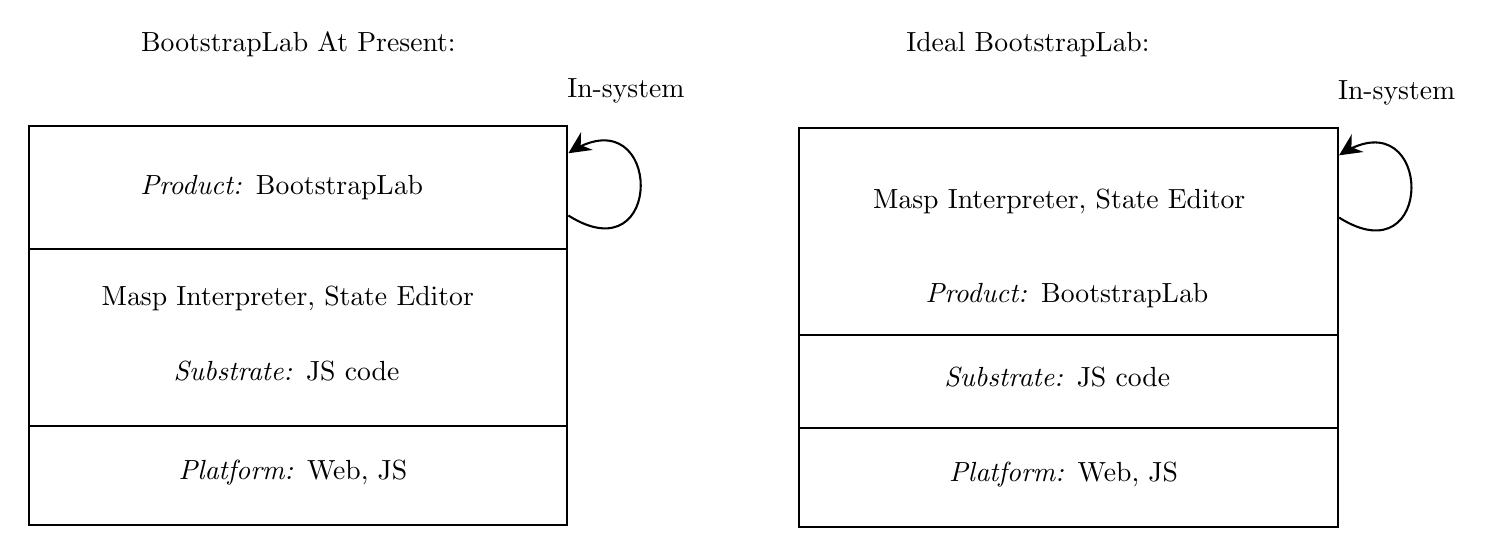
\begin{tikzpicture}[x=0.75pt,y=0.75pt,yscale=-1,xscale=1]
%uncomment if require: \path (0,302); %set diagram left start at 0, and has height of 302

%Shape: Rectangle [id:dp005746865399147039] 
\draw   (47,76.33) -- (306.33,76.33) -- (306.33,268.33) -- (47,268.33) -- cycle ;
%Straight Lines [id:da9945796961134794] 
\draw    (47,135.33) -- (307,135.33) ;
%Straight Lines [id:da675295141305357] 
\draw    (47,220.67) -- (307,220.67) ;
%Curve Lines [id:da12218560646601695] 
\draw    (307,119.33) .. controls (353.79,148.88) and (352.55,62.01) .. (309.02,88.06) ;
\draw [shift={(307,89.33)}, rotate = 326.6] [fill={rgb, 255:red, 0; green, 0; blue, 0 }  ][line width=0.08]  [draw opacity=0] (10.72,-5.15) -- (0,0) -- (10.72,5.15) -- (7.12,0) -- cycle    ;
%Shape: Rectangle [id:dp7917955958295702] 
\draw   (418.33,77.33) -- (677.67,77.33) -- (677.67,269.33) -- (418.33,269.33) -- cycle ;
%Straight Lines [id:da38902877975940764] 
\draw    (418.33,177) -- (678.33,177) ;
%Straight Lines [id:da4798892255665692] 
\draw    (418.33,221.67) -- (678.33,221.67) ;
%Curve Lines [id:da1475424514703748] 
\draw    (678.33,120.33) .. controls (725.12,149.88) and (723.88,63.01) .. (680.35,89.06) ;
\draw [shift={(678.33,90.33)}, rotate = 326.6] [fill={rgb, 255:red, 0; green, 0; blue, 0 }  ][line width=0.08]  [draw opacity=0] (10.72,-5.15) -- (0,0) -- (10.72,5.15) -- (7.12,0) -- cycle    ;

% Text Node
\draw (117.67,235.67) node [anchor=north west][inner sep=0.75pt]  [font=\normalsize] [align=left] {\textit{Platform:} Web, JS};
% Text Node
\draw (115.33,188) node [anchor=north west][inner sep=0.75pt]  [font=\normalsize] [align=left] {\textit{Substrate:} JS code};
% Text Node
\draw (99.33,98.67) node [anchor=north west][inner sep=0.75pt]  [font=\normalsize] [align=left] {\textit{Product: }BootstrapLab};
% Text Node
\draw (305,52) node [anchor=north west][inner sep=0.75pt]  [font=\normalsize] [align=left] {In-system};
% Text Node
\draw (80.67,152) node [anchor=north west][inner sep=0.75pt]  [font=\normalsize] [align=left] {Masp Interpreter, State Editor};
% Text Node
\draw (489,236.67) node [anchor=north west][inner sep=0.75pt]  [font=\normalsize] [align=left] {\textit{Platform:} Web, JS};
% Text Node
\draw (486.67,191) node [anchor=north west][inner sep=0.75pt]  [font=\normalsize] [align=left] {\textit{Substrate:} JS code};
% Text Node
\draw (477.67,150.33) node [anchor=north west][inner sep=0.75pt]  [font=\normalsize] [align=left] {\textit{Product: }BootstrapLab};
% Text Node
\draw (676.33,53) node [anchor=north west][inner sep=0.75pt]  [font=\normalsize] [align=left] {In-system};
% Text Node
\draw (452.33,105) node [anchor=north west][inner sep=0.75pt]  [font=\normalsize] [align=left] {Masp Interpreter, State Editor};
% Text Node
\draw (99.67,29.33) node [anchor=north west][inner sep=0.75pt]  [font=\normalsize] [align=left] {BootstrapLab At Present:};
% Text Node
\draw (468.33,29.33) node [anchor=north west][inner sep=0.75pt]  [font=\normalsize] [align=left] {Ideal BootstrapLab:};


\end{tikzpicture}
